\documentclass[a4 paper]{article}

\usepackage[utf8]{inputenc}
\usepackage{graphicx}
\begin{document}

\section{Istorija i pioniri}

U 19. veku su se razvile mnoge teorije i kontrateorije o tome kako se električna energija može prenositi. Godine 1826, Andre-Mari Amper je otkrio vezu izmedju struje i magneta. Majkl Faradej je 1831. opisao svojim zakonom indukcije elektromotornu silu koja pokreće struju u petlji provodnika uz pomoć vremenski promenljivog magnetnog fluksa. Prenos električne energije bez žica su posmatrali mnogi pronalazači i eksperimentatori, ali nedostatak odgovarajuće teorije je nejasno pripisao ove pojave elektromagnetnoj indukciji.

Koncizno objašnjenje ovih fenomena dolazilo bi iz Maksvelovih jednačina iz 1860-ih Džejmsa Klerka Maksvela, uspostavljajući teoriju koja je ujedinila elektricitet i magnetizam sa elektromagnetizmom, predvidjajući postojanje elektromagnetnih talasa kao "bežičnog" nosioca elektromagnetne energije.
Nakon toga je usledila validacija teorije od strane Hajnriha Rudolfa Herca iz 1888. godine, koja je uključivala dokaze za radio talase.

Guljelmo Markoni je 1897. godine uspešno poslao Morseovu azbuku na rastojanje od 6 km.
Na slici 1 su prikazani inženjeri Britanske pošte kako pregledaju Markonijevu radio opremu tokom demonstracije na ostrvu Flat Holm, 13. maja 1897. Predajnik je u sredini, prijemnik ispod njega, a stub koji podržava žičanu antenu je vidljiv na vrhu.

\begin{figure}[h!]
    \centering
    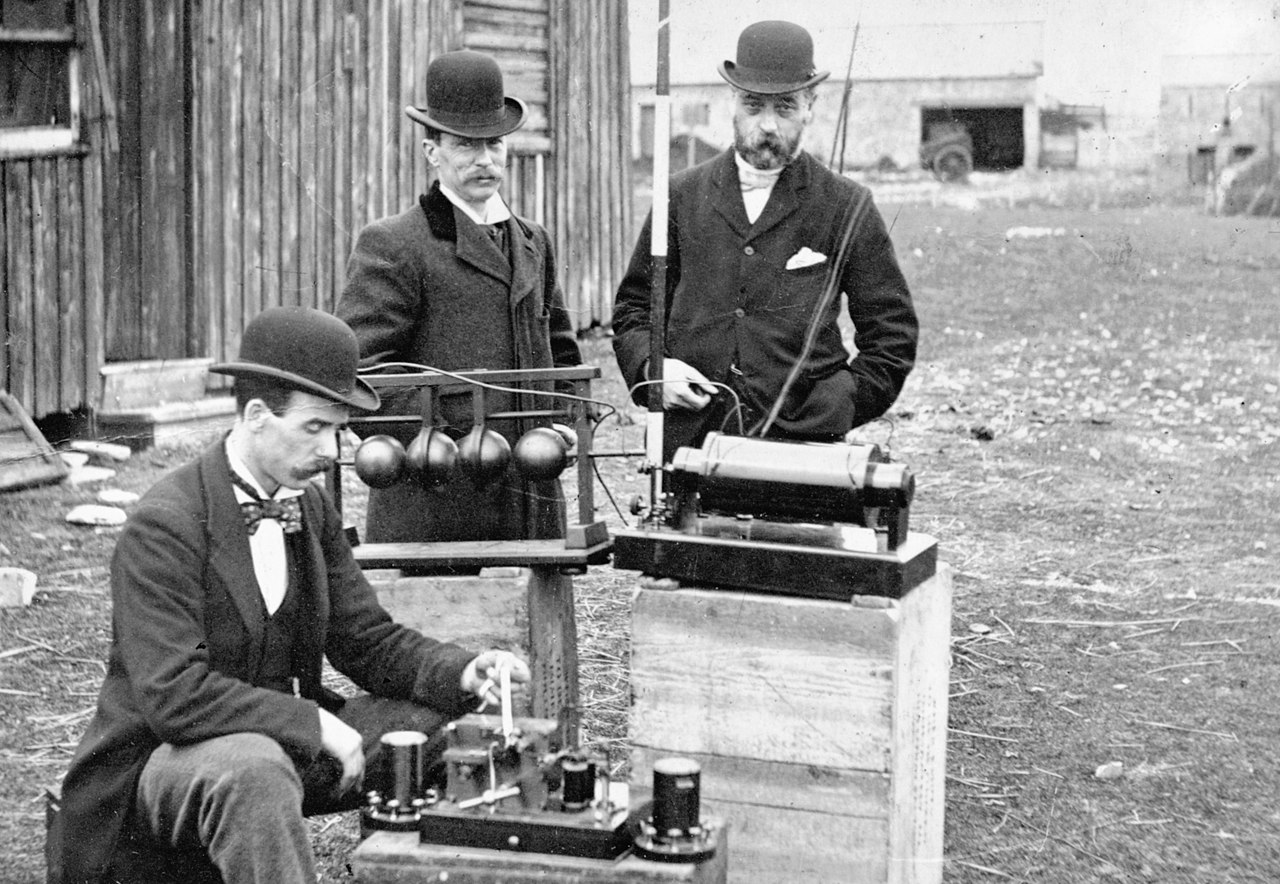
\includegraphics[scale=0.2]{Markoni.jpg}
    \caption{Markoni i inženjeri}
    \label{fig:my_labela}
\end{figure}



U medjuvremenu Tesla počinje ozbiljno proučavati ideju bežičnog prenosa električne energije. Njegova zamisao je bila da bežičnim putem svetu obezbedi besplatnu elekričnu energiju. 1893. osvetljava sijalicu bežičnim putem, a nedugo zatim započinje gradnju Vardenklif tornja
koji bi se koristio za prenos električne energije bežičnim putem na velike udaljenosti. Zbog velikih gubitaka projekt je ostao bez finansijskih sredstava i na kraju je ugašen. 

Vilijam Braun je 1964. pokazao model vazduhoplova na mikrotalasni pogon koji je svu
za let potrebnu energiju dobivao iz mikrotalasnih zraka. 
2003. NASA je letela prvim laserskim avionom. Motor malog modela aviona pokretala je električna energija koju su generisale fotoćelije iz snopa infracrvene svetlosti iz zemaljskog lasera, dok je kontrolni sistem držao laser uperen u avion.

\begin{figure}[h!]
    \centering
    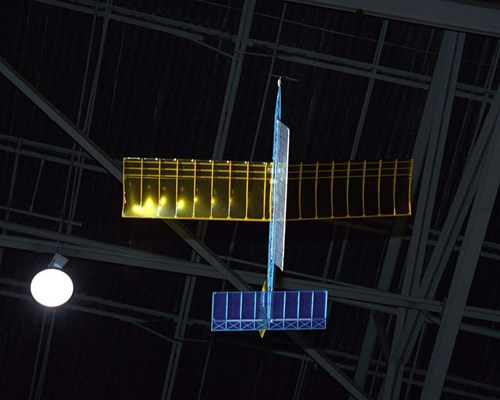
\includegraphics[scale=0.4]{aircraft.jpg}
    \caption{Prvi let NASA lasersog aviona}
    \label{fig:my_label}
\end{figure}


2008. Intel je pokazao da se može bežično poslati energija da bi se upalila sijalica sa efikasnošću prenosa 75 upešnih pokušaja na 100 pokušaja.


\end{document}

